%--------------------------URV DCSM ----------------------------%

\documentclass{dcsm}
\usepackage[spanish,english]{babel}

\usepackage{amsmath}
\usepackage{amsfonts}
\usepackage{latexsym}
\usepackage{epsfig}
\usepackage{graphicx}
\usepackage{url}

% If you use any other package, please indicate it to the organizers, when submitting the abstract.


\begin{document}
% This contribution must be written in English.
\selectlanguage{english}

\title*{
 Title of the abstract
}
\author{
 Name of the PhD Student \thanks{PhD advisor: Name of the advisor/s}
}

\institute{
 Department of Computer Engineering and Mathematics, Universitat Rovira i Virgili \\
 Tarragona, Spain \\
  \url{xxxxx.xxxx@urv.cat}
}

% Use "url.sty" for special characters in email address

\maketitle


%--------------------------------------------------------------%
%                    Content of the Abstract                   %
%--------------------------------------------------------------%


\section{Indications}

This is the template for the Book of Abstracts of the URV Workshop on
Computer Science and Mathematics.
It is important that you follow these guidelines.

The contribution to this workshop must have between 2 and 4 pages.
In case you need more pages, please contact before with the Workshop organizers.

The contribution should explain briefly the topic of your thesis to the readers.
The main aim of the workshop is to let other students know your work in a general way.
You can focus on some particular research issue also, if you consider it appropriate,
but take into account that this is not intended to be a contribution such as the usual
ones in specialized conferences (where you must show results, discussion, etc).

Prepare your contribution in Latex, using the file style \verb@dcsm.cls@ 
available at the web page of the workshop:
\url{http://deim.urv.cat/~dcsm/}.

\begin{verbatim}
\documentclass{dcsm}
\usepackage[spanish,english]{babel}
\usepackage{amsmath,amsfonts,latexsym}
\usepackage{epsfig,graphicx}
\usepackage{url}
\end{verbatim}


\section{Title of the section}
\label{sec_title}

% Use \ref{<label>} for cross references and
% \cite{<label>} for bibliographical references

You can divide the contribution into several sections and subsections.

\subsection{Title of the subsection}
\label{subs_title} Include here the text. With appropriate citations \cite{Kulick} to the related work \cite{Zhou} and \cite{BLMY}.

\section{Equations, Figures and Tables}

Equations, figures and tables will be centered. They must be numbered.
For example,

\begin{equation}
  \gamma(G \cap H)\ge \gamma(G) \cdot \gamma(H).
\end{equation}

Figures and tables must have a short caption, explaining briefly the content.
They must be put in the appropriate place in the text, like Figure \ref{fig_example}.
You can use color figures. Figures must be in EPS (Encapsulated PostScript) format.
See the Latex file provided in the web page of the workshop for the instructions.

%---------------------------------------------------------------------%
% The file must be introduced without "`eps"' extension because
% \LaTeX\ will search it automatically.
%---------------------------------------------------------------------%

\begin{figure}[ht]
  \centering
 \begin{center}
   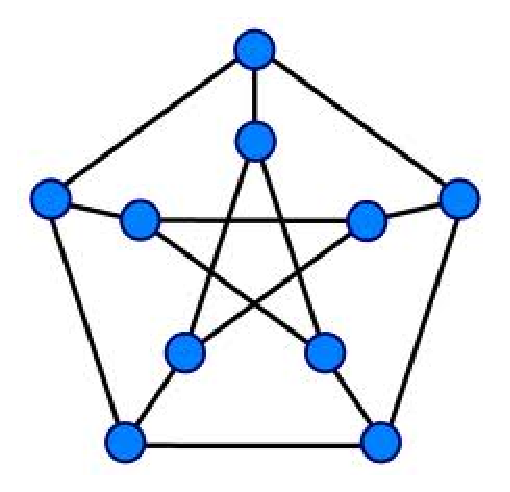
\includegraphics[width=.4\textwidth]{images}
 \end{center}
 \caption{Short caption, explaining the figure meaning.}
 \label{fig_example}
\end{figure}

Table \ref{tab_example} shows the format of tables in this document, in case you need them.


\begin{table}[ht]
	\centering
		\begin{tabular}{|ccc|}
       \hline
           first & second & third  \\
	     \hline
        1 & 2 & 3 \\
        4 & 5 & ... \\
  \hline
		\end{tabular}
 \caption{Short caption, explaining the table content.}
 \label{tab_example}
\end{table}



\subsection{Mathematics}

Although the aim of the contribution is to present an overall idea of your current work,
you may introduce some definitions or equations if you require them.
Use the following Latex commands \cite{Lamport}:


\begin{verbatim}
\begin{lemma}       ... \end{lemma}
\begin{proposition} ... \end{proposition}
\begin{theorem}     ... \end{theorem}
\begin{corollary}   ... \end{corollary}
\begin{conjecture}  ... \end{conjecture}
\begin{proof} ... \qed \end{proof}
\begin{example} ... \end{example}
\begin{note}    ... \end{note}
\begin{remark}  ... \end{remark}
\end{verbatim}




\section{Submission of the abstract}

A PDF version of the abstract must be submitted via EasyChair platform. Please, follow the instructions that appear in the workshop website.

The images and the latex source must be sent by email to dcsm@urv.cat. Send a ZIP file with all the font files in Latex, including figures. The name of the file must be the first surname of the PhD student.

The deadline for submission is {\bf June 23th, 2017}.

\section{Indications about the references}
The reference section must be ordered alphabetically. Please consider the example provided in this document for formatting the references.

\begin{acknowledgement}
Include here the acknowledgments (e.g. financial entities that support this work).
PhD students with a grant must indicate clearly who is providing the grant.
\end{acknowledgement}
\begin{thebibliography}{1}


\bibitem{BLMY}
M.~Ba\v ca, Y. Lin M.~Miller and M.Z. Youssef.
\newblock Edge-antimagic graphs.
\newblock {\em Discrete Math.}, 307(11--12):1232--1244, 2007.

\bibitem{Kulick}
J. Kulick, M. Toussaint, T. Lang, M. Lopes.
\newblock Active learning for teaching a robot grounded relational symbols.
\newblock  {\em Proc. 23rd. Int. Joint Conference on Artificial Intelligence}, 1451--1457, Beijing, China, 2013,


\bibitem{Lamport}
L. Lamport.
\newblock {\em LaTeX User's Guide and Document Reference Manual}.
\newblock Addison-Wesley Publishing Company, Reading, Massachusetts, 1986.


\bibitem{Zhou}
C.V. Zhou, C. Leckie, S. Karunasekera.
\newblock  A survey of coordinated attacks and collaborative intrusion detection.
\newblock  {\em Computers and Security}, 29(1):124--140, 2010.


\end{thebibliography}

\end{document}
%--------------------------------------------------------------%
%--------------------------------------------------------------%
